\section{Использование коллекций}

\textbf{Задание:} Создать словарь, состоящий из строк. В качестве ключа выступает фамилия, в качестве значения — должность. Вывести на экран фамилии людей, занимающих данную должность. 
Вывести должность, занимаемую данным человеком.
Вид окна представлен на рисунке \ref{fig:task7_form}.
\begin{figure}[H]
    \centering
    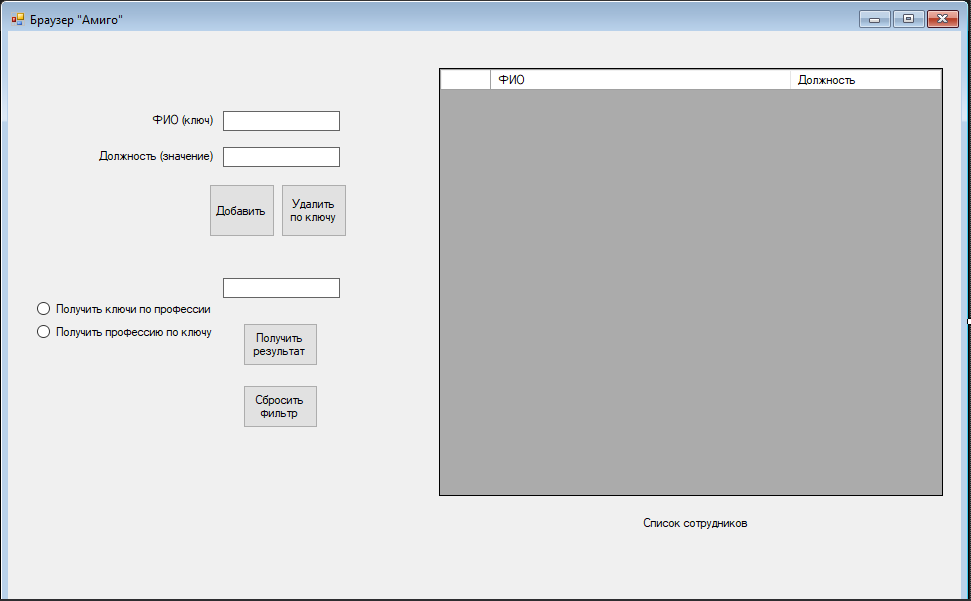
\includegraphics[scale=0.7]{task7/form.png}
    \caption{Внешний вид формы программы}
    \label{fig:task7_form}
\end{figure}
У элементов изменены значения некоторых атрибутов. 
Значения измененных атрибутов представлены в таблице \ref{table:params7}.
\begin{longtable}{|l|l|}
    Наименование атрибута & Значение\cr\hline
    \multicolumn{2}{|l|}{Для формы}\cr\hline
    \verb"Text" & \verb"Браузер "Амиго""\cr\hline
    \verb"FormBorderStyle" & \verb"FixedSingle"\cr\hline
    \verb"MaximizeBox" & \verb"False"\cr\hline
    \multicolumn{2}{|l|}{Для надписи ФИО}\cr\hline
    \verb"(Name)" & \verb"NameLabel"\cr\hline
    \verb"Text" & \verb"ФИО (ключ)"\cr\hline
    \multicolumn{2}{|l|}{Для текстового поля должности}\cr\hline
    \verb"(Name)" & \verb"PositionTextBox"\cr\hline
    \multicolumn{2}{|l|}{Для текстового поля ФИО}\cr\hline
    \verb"(Name)" & \verb"NameTextBox"\cr\hline
    \multicolumn{2}{|l|}{Для надписи должности}\cr\hline
    \verb"(Name)" & \verb"PositionLabel"\cr\hline
    \verb"Text" & \verb"Должность(значение)"\cr\hline
    \multicolumn{2}{|l|}{Для надписи к таблице}\cr\hline
    \verb"(Name)" & \verb"resultLabel"\cr\hline
    \verb"Text" & \verb"Список сотрудников"\cr\hline
    \multicolumn{2}{|l|}{Для кнопки добавления значения по ключу}\cr\hline
    \verb"(Name)" & \verb"AddBtn"\cr\hline
    \verb"Text" & \verb"Добавить"\cr\hline
    \multicolumn{2}{|l|}{Для кнопки удаления значения по ключу}\cr\hline
    \verb"(Name)" & \verb"RemoveBtn"\cr\hline
    \verb"Text" & \verb"Добавить"\cr\hline
    \multicolumn{2}{|l|}{Для текстового поля результата}\cr\hline
    \verb"(Name)" & \verb"ResultTextBox"\cr\hline
    \multicolumn{2}{|l|}{Для радиокнопки ключа по профессии}\cr\hline
    \verb"(Name)" & \verb"GetNamesBtn"\cr\hline
    \verb"Text" & \verb"Получить ключи по профессии"\cr\hline
    \multicolumn{2}{|l|}{Для радиокнопки профессии по ключу }\cr\hline
    \verb"(Name)" & \verb"GetPositionBtn"\cr\hline
    \verb"Text" & \verb"Получить профессию по ключу"\cr\hline
    \multicolumn{2}{|l|}{Для кнопки получения результата}\cr\hline
    \verb"(Name)" & \verb"ResultBtn"\cr\hline
    \verb"Text" & \verb"Получить результат"\cr\hline
    \multicolumn{2}{|l|}{Для кнопки сброса}\cr\hline
    \verb"(Name)" & \verb"ResetBtn"\cr\hline
    \verb"Text" & \verb"Сбросить фильтр"\cr\hline
    \multicolumn{2}{|l|}{Для обработчика ошибок}\cr\hline
    \verb"(Name)" & \verb"errorProvider1"\cr\hline
    \caption{Значения атрибутов элементов в приложении <<Матричный калькулятор}
    \label{table:params7}
\end{longtable}
Программа написана с использованием контейнеров из \verb|.NET framework| и
работы с ними соответственно назначению кнопки. Ниже приведен пример работы
функции добавления элемента по ключу:
\begin{minted}[fontsize=\small, breaklines=true, style=bw, linenos]{cpp}
private: System::Void AddBtn_Click(System::Object^ sender, System::EventArgs^ e) { // Добавление пары ключ - значение
	String^ name = NameTextBox->Text->ToString();
	String^ position = PosTextBox->Text->ToString();
	if (name == String::Empty || position == String::Empty) { // Если что-то не ввели - сообщим об этом
		errorProvider1->SetError(AddBtn, "Недопустимые значения");
		return;
	}
	if (!d.ContainsKey(name)) { // Если ключа нет, добавим
		d.Add(name, position);
		System::Collections::Generic::List<String^>^ lst = gcnew System::Collections::Generic::List<String^>(); // Создадим новый объект
		if (!p.ContainsKey(position)) 
			p.Add(position, lst);
		p[position]->Add(name); // Добавим в лист по этому ключу новое значение
		gridResult->Rows->Add(1);
		int _row = gridResult->RowCount;
		auto ResultPair = System::Collections::Generic::KeyValuePair<String^, String^>(name, position);
		FillRowWithDict(gridResult->Rows[_row - 1], ResultPair);
		}	
	}
};
\end{minted}
После запуска приложения открывается следующее окно (см. рисунок \ref{fig:exec7})
\begin{figure}[H]
    \centering
    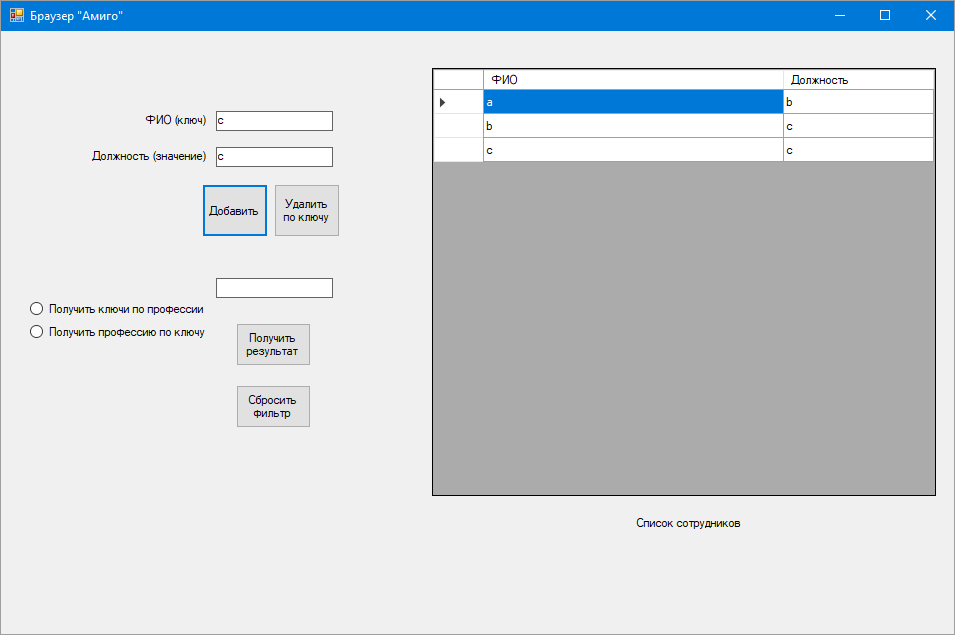
\includegraphics[scale=0.4]{task7/result3.png}
    \caption{Состояние приложения после добавление нескольких элементов по ключу}
    \label{fig:exec7}
\end{figure}
Ниже приведен пример работы программы:
После запуска приложения открывается следующее окно (см. рисунки \ref{fig:result7},\ref{fig:result71})
\begin{figure}[H]
    \centering
    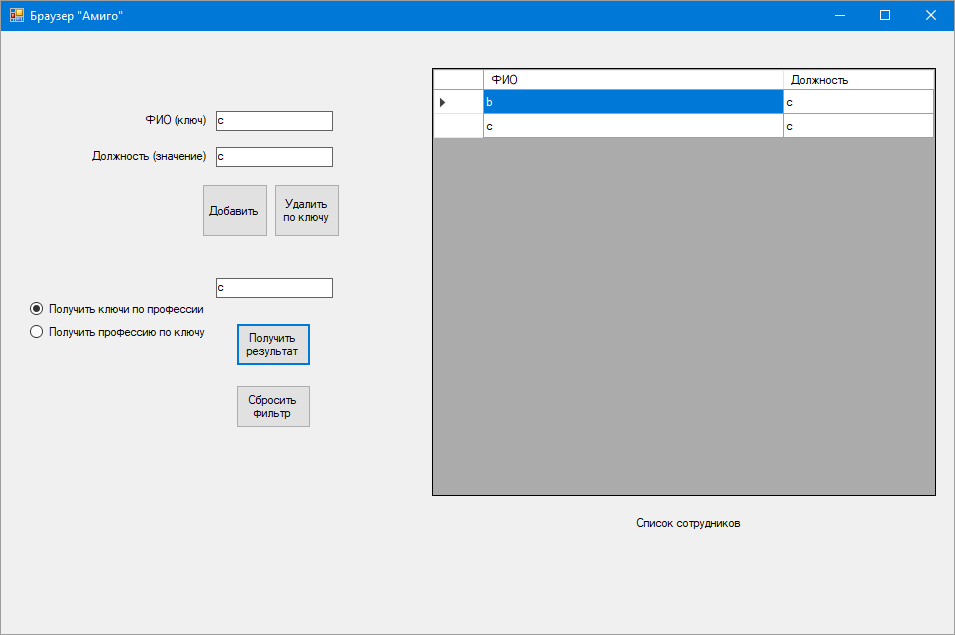
\includegraphics[scale=0.4]{task7/result4.png}
    \caption{Результат поиска по значению}
    \label{fig:result7}
\end{figure}
\begin{figure}[H]
    \centering
    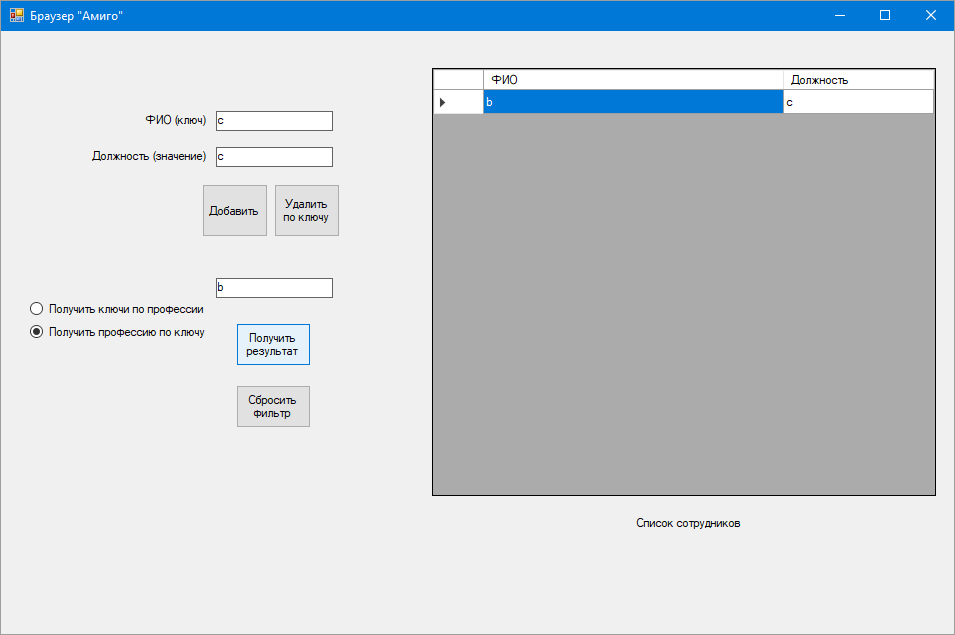
\includegraphics[scale=0.4]{task7/result5.png}
    \caption{Результат поиска по ключу}
    \label{fig:result71}
\end{figure}
В случае, если соответствующие поля не заполнены, выполнение программы
игнорируется.

Полный код программы приведен в приложении \ref{app:repos}.

